In this case, we consider $r_0 = 0$. 

\begin{center}
	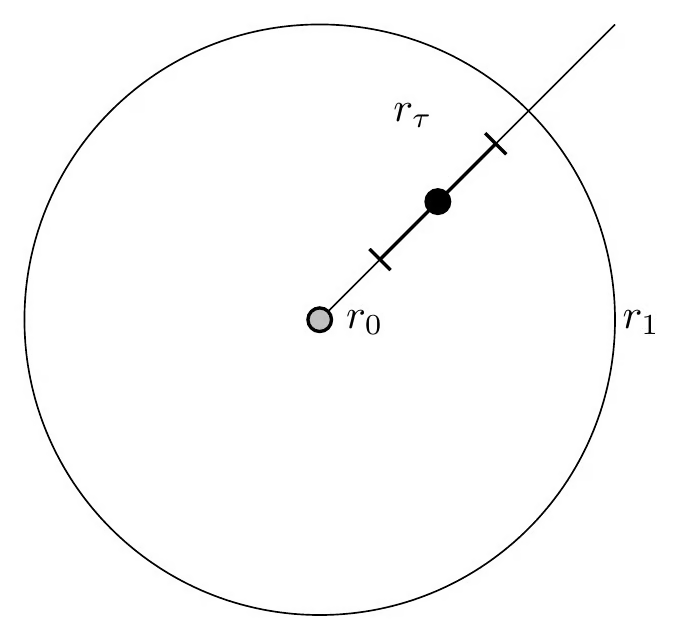
\includegraphics[width=.4\linewidth]{Assets/diskfar.png}
	\hspace{.15\linewidth}
	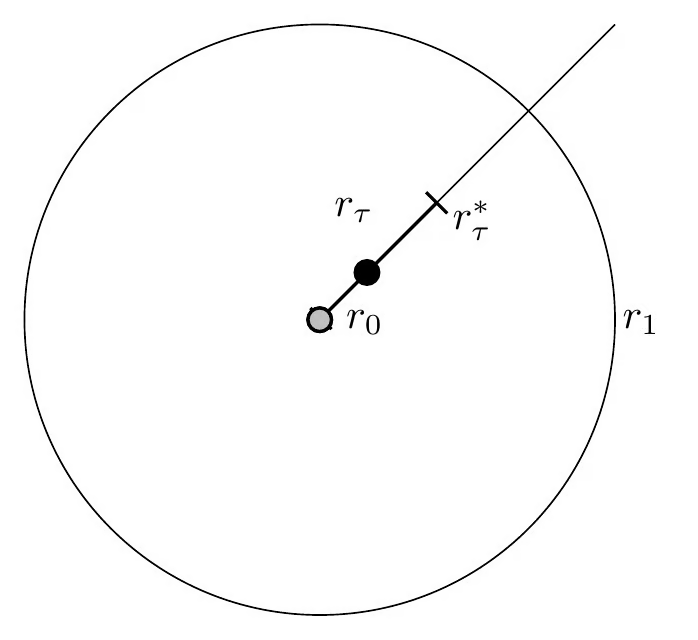
\includegraphics[width=.4\linewidth]{Assets/diskclose.png}
\end{center}

\subsubsection{Asymptotic for the orthogonal polynomial}

In the asymptotic expansions of $h_j$, one should distinguish the following two cases depending on a small constant $\epsilon > 0$. 
\begin{itemize}
	\item Case 1: $r_{j/N} >> N^{-\epsilon}$. For the annular droplet case where $r_0 > 0$, this case covers all $j = 0, 1, \cdots , N-1$. On the other hand, for the disc droplet case where $r_0 = 0$, this case covers only $j = m_N, m_N + 1, \cdots , N-1$ for $m_N = N^\epsilon$ with some $\epsilon > 0$;
	\item $r_{j/N} << N^{-\epsilon}$. This covers the remaining disc droplet case with $j = 0, 1, \cdots, m_N-1$. Notably, the asymptotic expansion involves gamma functions in this case. 
\end{itemize}

We separate this in two proofs, the first one for $j = m_N, m_N + 1, \cdots, N-1$  is very similar to our previous proof. To actually expand on the details, we need some useful facts. \textcolor{red}{First, recall tat $r_{\tau}$ satisfies $r_\tau = \Boh(\tau^{\frac{1}{2}})$ as $\tau \rightarrow 0$}. Note also that for $d \geq 1$, we can choose $C_1$ a constant uniformly for all $\tau$ and write
\begin{equation}
	|V^{(d)}_\tau(r_\tau)| = |q^{(d)}(r_\tau) + (-1)^{d} 2 \tau (d-1)! r_\tau^{-d} | \leq C_1 (1 + \tau^{-\frac{d}{2} + 1}).
\end{equation} 
We then star as usual dividing the integral into two parts
\begin{align}
	h_j & = \int_{0}^{\infty} 2 r^{2j + 1} \ee^{-N q(r)} \dd r = \int_{0}^{\infty} 2 r \ee^{-N V_{\tau(j)} (r)} \dd r \\
	&= \int_{r_{\tau(j)} - \delta_N}^{r_{\tau(j)} + \delta_N} 2 r \ee^{-N V_{\tau(j)}(r)} \dd r+ \int_{|r - r_{\tau(j)} > \delta_N} 2 r \ee^{-NV_{\tau(j)}(r)} \dd r
\end{align}
and now we have two integrals to solve. Let's star with the outer integral, which we should be able to control the growth. For $m_N \leq j < N$, we have
\begin{equation}
	r_{\tau(j + 1/2)} - r_{\tau(j)} = \Boh((jN)^{-\frac{1}{2}}).
\end{equation}
Since the potential is increasing in $(r_\tau, \infty)$, the Taylor series expansion for $V_\tau$ is for all $r > r_{\tau(j)} + \delta_N$
\begin{align}
	V_{\tau(j + 1/2)}(r) & \geq V_{\tau(j + 1/2)}(r) \\
	& = V_{\tau(j + 1/2)}(r_{\tau(j + 1/2)}) + \frac{1}{2} V^{(2)}_{\tau(j + 1/2)}(r_{\tau(j + 1/2)}) (r_{\tau(j)}) + \delta_N - r_{\tau(j + 1/2)})^2 + \Boh(\tau(j)^{-1/2} \delta^3_N).
\end{align}
where $\Boh(\tau(j)^{-1/2} \delta^3_N) = \Boh(N^{-1} j^{-1/2}(\log(N))^3)$. Similarly, since $V_{\tau}$ is decreasing in $(0, r_\tau)$, we have for all $r < r_{\tau(j)} - \delta_N$
\begin{align}
	V_{\tau(j + 1/2)}(r) & \geq V_{\tau(j - 1/2)}(r) \\
	& = V_{\tau(j + 1/2)}(r_{\tau(j + 1/2)}) + \frac{1}{2} V^{(2)}_{\tau(j + 1/2)}(r_{\tau(j + 1/2)}) (r_{\tau(j)}) - \delta_N - r_{\tau(j + 1/2)})^2 + \Boh(\tau(j)^{-1/2} \delta^3_N).
\end{align}
Using the Taylor series for $V_\tau$ again, we have
\begin{align}
	V_{\tau(j+1/2)}(r_{\tau(j+1/2)}) - V_{\tau(j)}(r_{\tau(j)}) & = V_{\tau(j)}(r_{\tau(j+1/2)}) - V_{\tau(j)}(r_{\tau(j)}) - \frac{1}{N} \log r_{\tau(j+1/2)} \\
	& = \Boh((jN)^{-1})  - \frac{1}{N} \log r_{\tau(j+1/2)}
\end{align}
Thus, if follows from the last two inequalities that
\begin{align}
	\ee^{N V_{\tau(j)}(r_{\tau(j)})} \int_{|r - r_{\tau(j)}| > \delta_N} 2 r^{2j+1} \ee^{-N q(r)} \dd r & = \int_{|r - r_{\tau(j)}| > \delta_N} 2 \ee^{-N \left( V_{\tau(j + 1/2)}(r) - V_{\tau(j)}(r_{\tau(j)}) \right)} \dd r \\
	& \leq \ee^{-c_1 (\log(N))^2} \ee^{\frac{N-M}{N} \log(r_{\tau(j+1/2)})}  \int_{|r - r_{\tau(j)}| > \delta_N} 2 \ee^{-M \left( V_{\tau(j + 1/2)}(r) - V_{\tau(j)}(r_{\tau(j)}) \right)} \dd r = \Boh(\ee^{c_2 (\log(N))^2})
\end{align}
for some constants $c_1, c_2 > 0$. We now need to examine the integral near the critical point. That is, 
\begin{align}
	& \int_{r_{\tau(j)} - \delta_N}^{r_{\tau(j)} + \delta_N} 2r \ee^{-N V_{\tau(j)}} \dd r \\
	& =  \ee^{-N V_{\tau(j)}(r_{\tau(j)})} \int_{-\delta_N}^{\delta_N} 2(r_{\tau(j)} + t) \ee^{-N \left( \frac{1}{2} V^{(2)}_{\tau(j)}(r_{\tau(j)}) (t)^2 + \frac{1}{3!} V^{(3)}_{\tau(j)}(r_{\tau(j)}) (t)^3 + \frac{1}{4!} V^{(4)}_{\tau(j)}(r_{\tau(j)}) (t)^4 + \Boh(\tau(j)^{-\frac{3}{2}}  t^5) \right)} \dd t \\
	&  =  \ee^{-N V_{\tau(j)}(r_{\tau(j)})}  \int_{-\sqrt{N} \delta_N}^{\sqrt{N} \delta_N} 2 \ee^{-2\Delta Q(r_{\tau(j)}) t^2} (r_{\tau(j)} + \frac{t}{\sqrt{N}})  \left(  1 - \frac{V^{(3)}_{\tau(j)}(r_{\tau(j)}) (t)^3 }{6 \sqrt{N}} - \frac{V^{(4)}_{\tau(j)}(r_{\tau(j)}) (t)^4}{24 N} + \frac{V^{(3)}_{\tau(j)}(r_{\tau(j)})^2 (t)^6}{72 N} + \epsilon'_{N,1} \right) \dd t
\end{align}
where  $\epsilon_{N,1} = \Boh(j^{-\frac{3}{2}} (\log N)^\alpha)$ for some $\alpha > 0$.

Now, for $j \leq m_N$, we need to define some $r^*_\tau \deff r_\tau \log(N)$ from which we separate the integral in a important part close to the origin and another part which has a lesser order. Consider
\begin{equation}
	h_j = \int_{0}^{\infty} 2r^{2j+1} \ee^{-N q(r)} \dd r =\int_{0}^{r^*_{\tau(j+\frac{1}{2})}} 2r^{2j+1} \ee^{-N q(r)} \dd r + \int_{r^*_{\tau(j+\frac{1}{2})}}^{\infty} 2r^{2j+1} \ee^{-N q(r)} \dd r
\end{equation}
\textcolor{red}{Due to strict subharmonicity of Q in a neighborhood of the droplet, $r_\tau$ satisfies $r_\tau = \Boh (\tau^{\frac{1}{2}})$ as $\tau \rightarrow 0$}. Since $V_\tau$ has a global minimum at $r = r_\tau$ and increases for larger values, for all $r > r^*_{\tau(j + 1/2)}$ we have
\begin{align}
	V_{\tau(j+1/2)}(r) & \geq V_{\tau(j+1/2)}(r)(r^*_{\tau(j+1/2)}) = q(r^*_{\tau(j+1/2)}) - \frac{2j + 1}{N} \log(r^*_{\tau(j+1/2)}) \\
	& = q(0) + \frac{1}{2} q^{(2)}(0)(r^*_{\tau(j+1/2)})^2 - \frac{2j + 1}{N} \log(r^*_{\tau(j+1/2)}) + \Boh(r^*_{\tau(j+1/2)})^3.
\end{align}
Remember that $q'(0) = 0$ and $\Delta Q(z) \in (0, \infty)$ near the origin. Using this inequality,
\begin{align}
	& \ee^{N q(0)} \int_{r^*_{\tau(j+\frac{1}{2})}}^{\infty} 2r^{2j+1} \ee^{-N q(r)} \dd r = \int_{r^*_{\tau(j+\frac{1}{2})}}^{\infty} 2 \ee^{-N (V_{\tau(j+1/2)}(r) q(0))} \dd r \\
	& \leq \ee^{-c_1 (N-M) (r^*_{\tau(j+\frac{1}{2})})^2} (r^*_{\tau(j+\frac{1}{2})})^{(2j+1) \frac{N-M}{N}} \int_{r^*_{\tau(j+\frac{1}{2})}}^{\infty} 2 \ee^{-M (V_{\tau(j+1/2)}(r) q(0))} \dd r \deff \epsilon_N(j)
\end{align}
for some $c_1 > 0$ and $M$ as given in the other proof, such that the appropriate integral converges. Since $r_\tau = \Boh(\tau^{\frac{1}{2}})$, there is a constant $c_2 > 0$ such that
\begin{equation}
	\epsilon_N(j) = \Boh\left( (r^*_{\tau(j+\frac{1}{2})})^{(2j+1) \frac{N-M}{N}} \ee^{-c_2 (j + \frac{1}{2}) (\log N)^2} \right) = \Boh\left( (\frac{2j+1}{2N} (\log(N))^2)^{(2j+1) \frac{N-M}{N}} \ee^{-c_2 (j + \frac{1}{2}) (\log N)^2} \right)
\end{equation}
Therefore we obtain
\begin{align}
	h_j & = \int_{0}^{\infty} 2r^{2j+1} \ee^{-N q(r)} \dd r = \int_{0}^{r^*_{\tau(j+\frac{1}{2})}} 2r^{2j+1} \ee^{-N q(r)} \dd + \ee^{-N q(0)} \epsilon_N(j) \\
	& = \int_{0}^{r^*_{\tau(j+\frac{1}{2})}} 2r^{2j+1} \ee^{-N \left( q(0) + \frac{1}{2} q^{(2)}(0) r^2 \right) + \Boh(N(r^*_{\tau(j+\frac{1}{2})})^3)} \dd  r + \ee^{-N q(0)} \epsilon_N(j) \\
	& =  \ee^{-N q(0)} \left[ N{-(j+1)} \int_{0}^{r^*_{\tau(j+\frac{1}{2})}} 2r^{2j+1} \ee^{-\frac{1}{2} q^{(2)}(0) r^2} \dd r \left( 1 + \Boh(N(r^*_{\tau(j+\frac{1}{2})})^3) \right)+ \epsilon_N(j) \right] \\
	&=  \ee^{-N q(0)} \left[ N{-(j+1)} \Gamma(j+1)(\frac{1}{2} q^{(2)}(0))^{-(j+1)} \left( 1 + \Boh(N^{-\frac{1}{2}} (j+\frac{1}{2})^{\frac{3}{2}} (\log N)^3) \right)+ \epsilon_N(j) \right]
\end{align}
and this completes this part of the proof.  

\subsubsection{Asymptotics on the Summation}

Now we complete the case calculating, using the results above,
\begin{equation}
	\sum_{j=0}^{N} \log(h_j) = \sum_{j=0}^{m_N - 1} \log(h_j)  + \sum_{j=m_N}^{N - 1} \log(h_j) 
\end{equation}
The first term in the right is easily determined, we need only to write
\begin{align}
	\sum_{j=0}^{m_N - 1} \log(h_j) & = -m_N N q(0) - \frac{m_N(m_N + 1)}{2} \left( \log(N) + \log\left( \frac{1}{2} q^{(2)}(0) \right) \right) + \log(G(m_N + 1)) + \Boh(N^{-\frac{1}{2}(1-5\epsilon)} (\log(N))^3) \\
	& = -m_N N q(0) - \frac{m_N(m_N + 1)}{2} \left( \log(N) + \log\left( \frac{1}{2} q^{(2)}(0) \right)  \right) +  \frac{m_N^2 \log(m_N)}{2} - \frac{3}{4} m_N^2 + \frac{\log(2\pi) m_N}{2} - \frac{\log(m_N)}{12} + \gamma'(-1)+ \Boh(m_N^{-2}+ N^{-\frac{1}{2}(1-5\epsilon)} (\log(N))^3)
\end{align}
where we have used the asymptotic for the G-Barnes function
\begin{equation}
	\log(G(z+1)) = \frac{z^2 \log(z)}{2} - \frac{3}{4} z^2 + \frac{\log(2\pi) z}{2} - \frac{\log(z)}{12} + \gamma'(-1) + \Boh(\frac{1}{z^2})
\end{equation}

The second summation is a bit more detailed, we use the previously defined
\begin{equation}
	\log(h_j) = -N V_{\tau(j)} (r_{\tau(j)}) + \frac{1}{2} \log{\left( \frac{2\pi r^2_{\tau(j)}}{N \Delta Q(r_{\tau(j)})} \right)} + \frac{1}{N} \mathfrak{B}_1(r_{\tau(j)}) + \Boh(j^{-\frac{3}{2}} (\log(N))^\alpha)
\end{equation}
and need to determine three things in order to get the summation,
\begin{align}
	& \sum_{j=m_N}^{N-1} V_{\tau(j)}(r_{\tau(j)}), \\
	& \sum_{j=m_N}^{N-1} \log \Delta Q(r_{\tau(j)}), \\
	&  \sum_{j=m_N}^{N-1} \log(r_{\tau(j)}).
\end{align}

For the first we proceed as before and perform the Euler-Maclaurin formula.
\begin{equation}
	\sum_{j=m_N}^{N-1} V_{\tau(j)}(r_{\tau(j)}) = \int_{m_N}^N V_{\tau(j)}(r_{\tau(j)})  \dd t - \frac{1}{2} \left( V_{\tau(N)}(r_{\tau(N)})  - V_{\tau(m_N)}(r_{\tau(m_N)}) \right) + \frac{1}{12} \left[ \partial_t V_{\tau(j)}(r_{\tau(j)}) |_{t=N} - \partial_t V_{\tau(j)}(r_{\tau(j)}) |_{t=m_N} \right] + \Boh(N^{-1-2\epsilon})
\end{equation}
where we used $\partial^3_t(V_{\tau(t)}(r_{\tau(t)})) |_{t=m_N} = \Boh(N^{-3} (\tau(m_N))^{-2}) = \Boh(m_N^{-2} N^{-1})$. The first term can be solved in a very similar way as before.
\begin{align}
	\int_{m_N}^{N} V_{\tau(j)}(r_{\tau(j)}) & = 2N \int_{r_\tau(m_N)}^{r_1} (q(s) - s q'(s) \log s) s \Delta Q(s) \dd s \\
	& = N \left( \frac{1}{2} \int_{S \backslash S_{\tau(m_N)}} Q \Delta Q \dd A - \log(r_1) + (\tau(m_N))^2 \log(r_{\tau(m_N)} + \frac{1}{2} \left( q(r_1) - \tau(m_N) q(r_{\tau(m_N)}) \right) \right) \\
	& = N I_Q[\mu_Q] - \frac{N}{2} \int_{S_{\tau(m_N)}} Q \Delta Q \dd A + \frac{m_N^2}{N} \log(r_{\tau(m_N)}) - \frac{m_N}{2} q(r_{\tau(m_N)}) 
\end{align}
where, \textcolor{red}{because 
	\begin{equation}
		r_\tau = \left(\frac{2 \tau}{q^{(2)}(0)} \right)^{\frac{1}{2}} + \Boh(\tau) = \left(\frac{\tau}{\Delta Q(0)} \right)^{\frac{1}{2}} + \Boh(\tau), \qquad \text{as} \quad \tau \rightarrow 0
\end{equation}}
we have that
\begin{equation}
	\log(r_{\tau(m_N)}) = \frac{1}{2} \log{\left(\frac{\tau(m_N)}{\Delta Q(0)}\right)} + \Boh(\tau(m_N)^{\frac{1}{2}}) = \frac{1}{2} \log{\left(\frac{\tau(m_N)}{\Delta Q(0)}\right)} + \Boh(N^{-\frac{1}{2}(1-\epsilon)}) 
\end{equation}
and
\begin{equation}
	q(r_{\tau(m_N)}) = q(0) + \frac{1}{2} q^{(2)}(0)(r_{\tau(m_N)})^2 + \Boh((\tau(m_N)^{\frac{3}{2}})) = q(0) + \tau(m_N) + \Boh(N^{-\frac{3}{2}(1 - \epsilon)})
\end{equation}